\documentclass[letterpaper, 10pt]{article}
\usepackage[utf8]{inputenc}
\usepackage{amsmath}
\usepackage{amsfonts}
\usepackage{amssymb}
\usepackage[letterpaper, margin=1in]{geometry}

\usepackage{pgfplots}
\usepackage{xcolor}
\usepackage{listings}
\usepackage{layouts}
\usepackage[section]{placeins}
\lstset{ 
	% language=Python,                	% choose the language of the code
	basicstyle=\ttfamily\footnotesize, 	% the size of the fonts that are used for the code
	numbers=left,                   	% where to put the line-numbers
	numberstyle=\ttfamily\footnotesize, % the size of the fonts that are used for the line-numbers
	stepnumber=1,                   	% the step between two line-numbers. If it is 1 each line will be numbered
	numbersep=5pt,                  	% how far the line-numbers are from the code
	backgroundcolor=\color{white}, 		% choose the background color. You must add \usepackage{color}
	showspaces=false,               	% show spaces adding particular underscores
	showstringspaces=false,         	% underline spaces within strings
	showtabs=false,                 	% show tabs within strings adding particular underscores
	frame=single,           			% adds a frame around the code
	tabsize=4,          				% sets default tabsize to 4 spaces
	captionpos=t,           			% sets the caption-position to bottom
	breaklines=true,        			% sets automatic line breaking
	breakatwhitespace=false,    		% sets if automatic breaks should only happen at whitespace
	escapeinside={\%*}{*)}          	% if you want to add a comment within your code
	% prebreak=\raisebox{0ex}[0ex][0ex]{\ensuremath{\hookleftarrow}})
}

% \pagenumbering{gobble}

\begin{document}
\section{Experiment 1}
\subsection{Small Batch Experiments}
\begin{figure}[h]
\centering
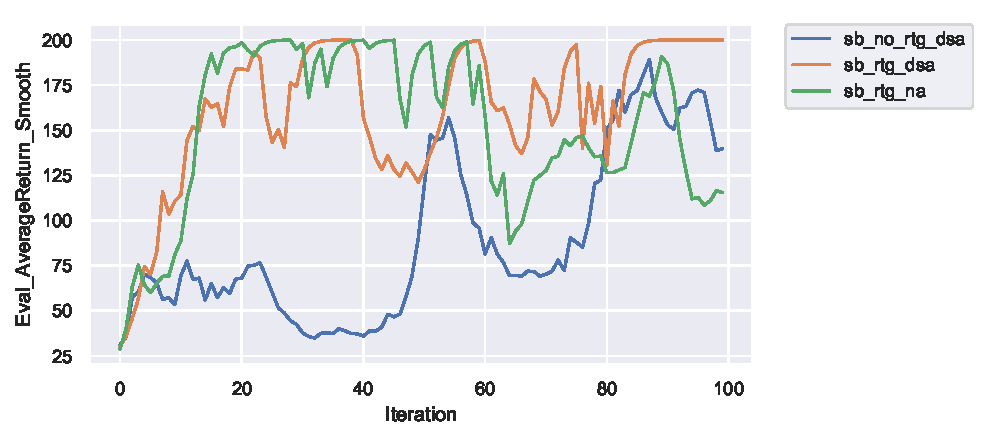
\includegraphics{figures/q1_sb.pdf}
\caption{Small Batch Experiments}
\end{figure}

\begin{lstlisting}[caption=Exact command line configurations]
python cs285/scripts/run_hw2.py --env_name CartPole-v0 -n 100 -b 1000 -dsa --exp_name q1_sb_no_rtg_dsa
python cs285/scripts/run_hw2.py --env_name CartPole-v0 -n 100 -b 1000 -rtg -dsa --exp_name q1_sb_rtg_dsa
python cs285/scripts/run_hw2.py --env_name CartPole-v0 -n 100 -b 1000 -rtg --exp_name q1_sb_rtg_na
\end{lstlisting}

The blue line used the trajectory-centric value estimator and did not standardize the advantages, which performed 
the worst. The orange line used the reward-to-go value estimator and did not standardize advantages, while the green line 
used the reward-to-go and did standardize advantages. The orange and green lines performed similarly, which seems to indicate 
that advantage standardization did not help that much. 

\newpage

\subsection{Large Batch Experiments}
\begin{figure}[h]
\centering
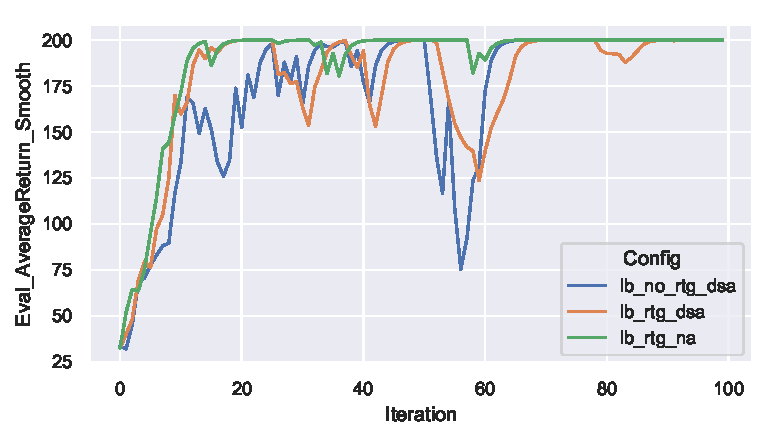
\includegraphics{figures/q1_lb.pdf}
\caption{Large Batch Experiments}
\end{figure}

In Figure 2, we can see the learning curve of the large batch experiments. The following commands were run:
\begin{lstlisting}[caption=Exact command line configurations]
python cs285/scripts/run_hw2.py --env_name CartPole-v0 -n 100 -b 5000 -dsa --exp_name q1_lb_no_rtg_dsa
python cs285/scripts/run_hw2.py --env_name CartPole-v0 -n 100 -b 5000 -rtg -dsa --exp_name q1_lb_rtg_dsa
python cs285/scripts/run_hw2.py --env_name CartPole-v0 -n 100 -b 5000 -rtg --exp_name q1_lb_rtg_na
\end{lstlisting}

The blue line had the trajectory-centric value estimator and did not standardize advantages. The orange line used the
reward-to-go and did not standardize advantages, while the green line used the reward-to-go and did standardize advantages.

Without advantage standardization, the reward-to-go had a better performance. In both the large and small batch experiments, the 
reward-to-go value estimator converged in fewer iterations than the trajectory-centric estimator. Advantage standardization 
did not seem to help, the reward-to-go experiments with and without advantage standardization seem to converge at roughly the
same rate. Larger batch sizes significantly helped the policy, as the experiments with larger batch sizes converged in fewer
iterations than the small batch size experiments.

\newpage

\section{Experiment 2: InvertedPendulum}

\begin{figure}[h]
\centering
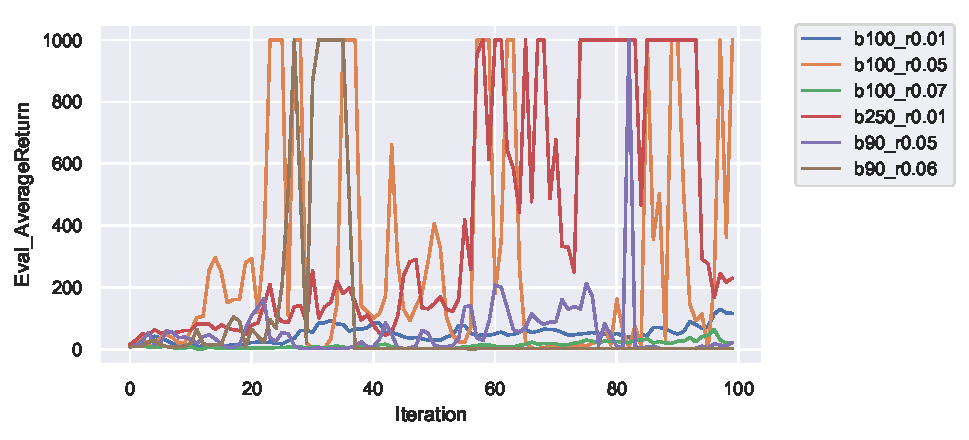
\includegraphics{figures/q2.pdf}
\caption{LunarLanderContinuous-v2}
\end{figure}

\begin{lstlisting}[caption=Exact command line configurations]
python cs285/scripts/run_hw2.py --env_name InvertedPendulum-v2 --ep_len 1000 --discount 0.9 -n 100 -l 2 -s 64 -b <b*> -lr <r*> -rtg --exp_name q2_b<b*>_r<r*>
\end{lstlisting}

The smallest batch size and largest learning rate I was able to get to converge to the optimum was 100 and 0.05 respectively. I 
used the above command except with \texttt{<b*>} replaced with 100 and \texttt{<r*>} replaced with 0.05. However, the policy
was still quite unstable, and deviations from those values would cause the policy to not converge at all. A batch size of 90
and learning rate of 0.05 did not converge and a batch size of 100 with a learning rate of 0.07 did not converge either. 

\newpage

\section{Experiment 3: LunarLander}

\begin{figure}[h]
\centering
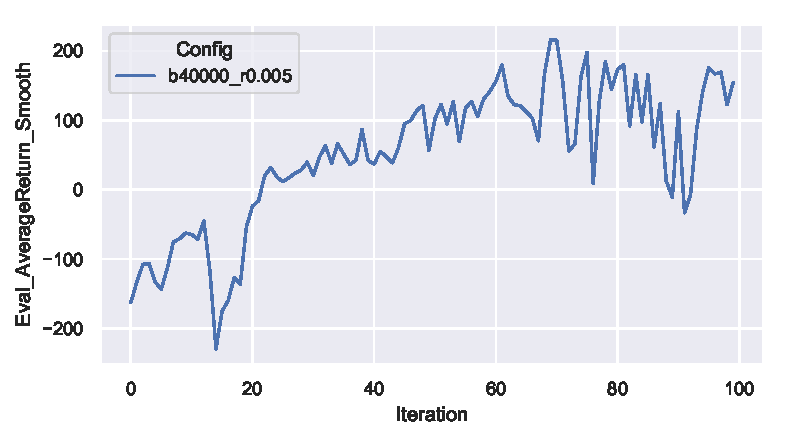
\includegraphics{figures/q3.pdf}
\caption{LunarLanderContinuous-v2}
\end{figure}

This experiment was run with the following command:
\begin{lstlisting}[caption=Exact command line configurations]
python cs285/scripts/run_hw2.py --env_name LunarLanderContinuous-v2 --ep_len 1000 --discount 0.99 -n 100 -l 2 -s 64 -b 40000 -lr 0.005 --reward_to_go --nn_baseline --exp_name q3_b40000_r0.005
\end{lstlisting}

\newpage
\section{Experiment 4: HalfCheetah}

\begin{figure}[h]
\centering
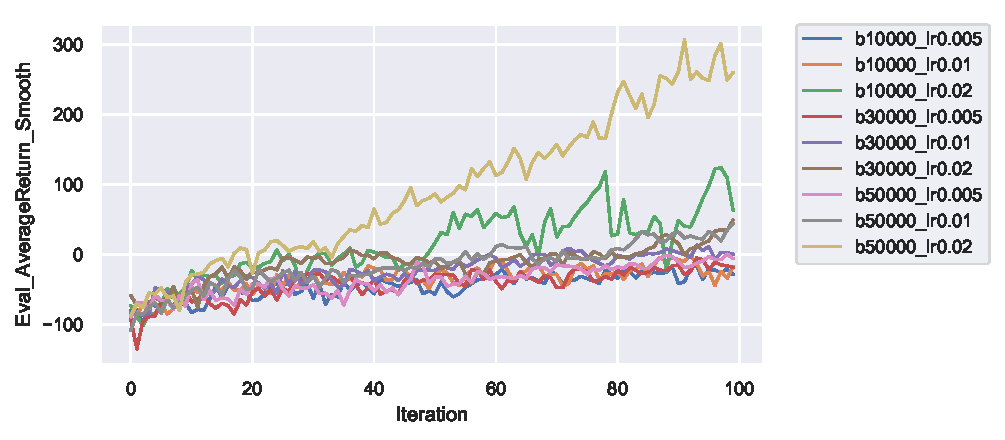
\includegraphics{figures/q4_search.pdf}
\caption{HalfCheetah Hyperparameter Search}
\end{figure}

\begin{lstlisting}[caption=Exact command line configurations]
python cs285/scripts/run_hw2.py --env_name HalfCheetah-v2 --ep_len 150 --discount 0.95 -n 100 -l 2 -s 32 -b 10000 -lr 0.005 -rtg --nn_baseline --exp_name q4_search_b10000_lr0.005_rtg_nnbaseline
python cs285/scripts/run_hw2.py --env_name HalfCheetah-v2 --ep_len 150 --discount 0.95 -n 100 -l 2 -s 32 -b 10000 -lr 0.01 -rtg --nn_baseline --exp_name q4_search_b10000_lr0.01_rtg_nnbaseline
python cs285/scripts/run_hw2.py --env_name HalfCheetah-v2 --ep_len 150 --discount 0.95 -n 100 -l 2 -s 32 -b 10000 -lr 0.02 -rtg --nn_baseline --exp_name q4_search_b10000_lr0.02_rtg_nnbaseline
python cs285/scripts/run_hw2.py --env_name HalfCheetah-v2 --ep_len 150 --discount 0.95 -n 100 -l 2 -s 32 -b 30000 -lr 0.005 -rtg --nn_baseline --exp_name q4_search_b30000_lr0.005_rtg_nnbaseline
python cs285/scripts/run_hw2.py --env_name HalfCheetah-v2 --ep_len 150 --discount 0.95 -n 100 -l 2 -s 32 -b 30000 -lr 0.01 -rtg --nn_baseline --exp_name q4_search_b30000_lr0.01_rtg_nnbaseline
python cs285/scripts/run_hw2.py --env_name HalfCheetah-v2 --ep_len 150 --discount 0.95 -n 100 -l 2 -s 32 -b 30000 -lr 0.02 -rtg --nn_baseline --exp_name q4_search_b30000_lr0.02_rtg_nnbaseline
python cs285/scripts/run_hw2.py --env_name HalfCheetah-v2 --ep_len 150 --discount 0.95 -n 100 -l 2 -s 32 -b 50000 -lr 0.005 -rtg --nn_baseline --exp_name q4_search_b50000_lr0.005_rtg_nnbaseline
python cs285/scripts/run_hw2.py --env_name HalfCheetah-v2 --ep_len 150 --discount 0.95 -n 100 -l 2 -s 32 -b 50000 -lr 0.01 -rtg --nn_baseline --exp_name q4_search_b50000_lr0.01_rtg_nnbaseline
python cs285/scripts/run_hw2.py --env_name HalfCheetah-v2 --ep_len 150 --discount 0.95 -n 100 -l 2 -s 32 -b 50000 -lr 0.02 -rtg --nn_baseline --exp_name q4_search_b50000_lr0.02_rtg_nnbaseline
\end{lstlisting}

As seen in the graph, the yellowish-green line, which corresponds with \texttt{batch\_size=50000} and \texttt{lr=0.02} performed
the best. Batch size alone did not have the same impact as a properly tuned learning rate. Of the experiments with
\texttt{batch\_size=50000}, only the one with \texttt{lr=0.02} performed noticeably better than the other experiments. The other
experiments with that batch size performed on par with the other experiments. Interestingly, the experiment with 
\texttt{batch\_size=10000} and \texttt{lr=0.02} performed better than nearly all of the other experiments (but not as well as
the one with \texttt{batch\_size=50000}), which indicates that a properly tuned learning rate has a larger effect on 
the performance of the policy. Since \texttt{batch\_size=50000} and \texttt{lr=0.02} performed the best, I ran the next
four experiments with those hyperparameter values, which is shown in the next figure.

\begin{figure}[h]
\centering
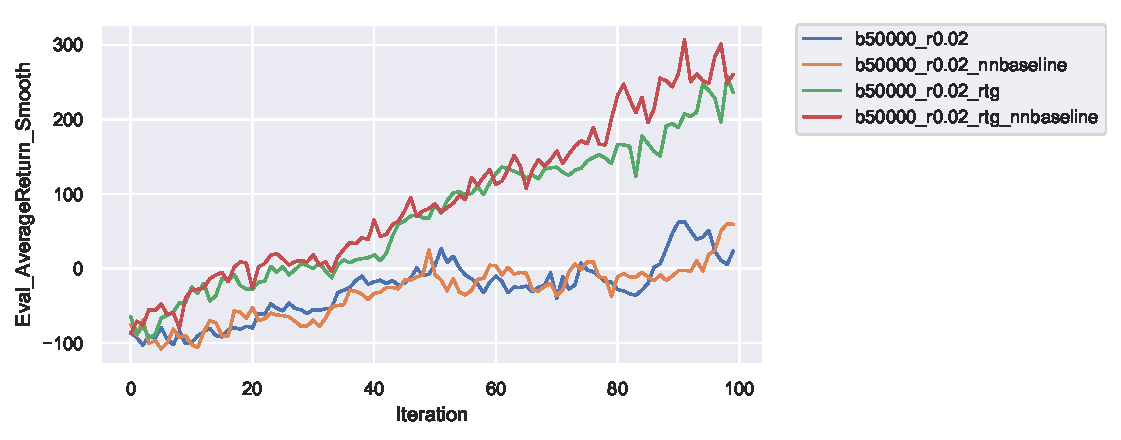
\includegraphics{figures/q4_optimal.pdf}
\caption{HalfCheetah Experiments}
\end{figure}

From the figure, we can see that the reward-to-go value estimator had a significant effect on the performance of the policy 
gradient. The two experiments with reward-to-go performed significantly better than the experiments that did not use it, and
the baseline only improved the policy slightly (maybe even not at all). 

\end{document}